\chapter{Experiments and Results}

In this chapter, the entire experimental process is presented, from the acquisition of the ground truth dataset (see section \ref{gt}), to the implementation, training and prediction phases of the \modelnameshort\ (see section \ref{impdet}), and finally to the results evaluation and analysis (see section \ref{expres}).

\section{Ground Truth}\label{gt}

Our ground truth dataset consists of satellite images and buildings' coordinates, which are used as inputs and labels respectively when training. In this project, all of the satellite images are collected from Google Static Maps API and all of the latitude and longitude coordinates of the polygon vertices of buildings are collected from OpenStreetMap. For details of the two APIs mentioned above, please refer to subsections \ref{apimap} and \ref{apiosm}.

As mentioned in section \ref{modmer}, the training phase of our model \modelnameshort\ requires two different kinds of ground truth dataset, areas with multiple bounding boxes for FPN and buildings with geometrical shapes for PolygonRNN, all of which are illustrated in subsection \ref{arebui}.

Since the whole dataset is collected from two different sources, the problem of inconsistency may exist. Subsection \ref{proble} describes details of the problems in the ground truth dataset, and subsection \ref{adjust} proposes a solution to adjust the shift between buildings' images and polygons.

\subsection{Google Static Maps API}\label{apimap}

Google Static Maps API\footnote{\lstinline{https://developers.google.com/maps/documentation/static-maps/}} provides an interface that implements maps as high-resolution images. Users can download customized map based on URL with different parameters, which is sent through a standard HTTPS request.

The parameters in URL includes the map type (satellite, roadmap, etc.), latitude and longitude coordinates of the image center, the resolution of the image, the zoom level, and the scale. For the usage of the Google Static Maps API, please refer to section \ref{app:apimap} in appendices. Figure \ref{fig:egsatellite} and \ref{fig:egroadmap} shows two types of images can be obtained by Google Static Maps API.

\begin{figure}[!h]
	\centering
	\subbottom[satellite image\label{fig:egsatellite}]
		{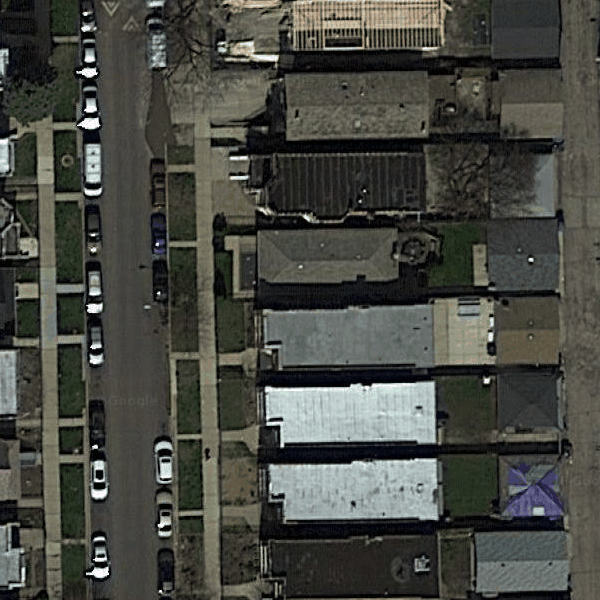
\includegraphics[width=0.328\textwidth]{4-00-0.png}}
	\subbottom[roadmap image\label{fig:egroadmap}]
		{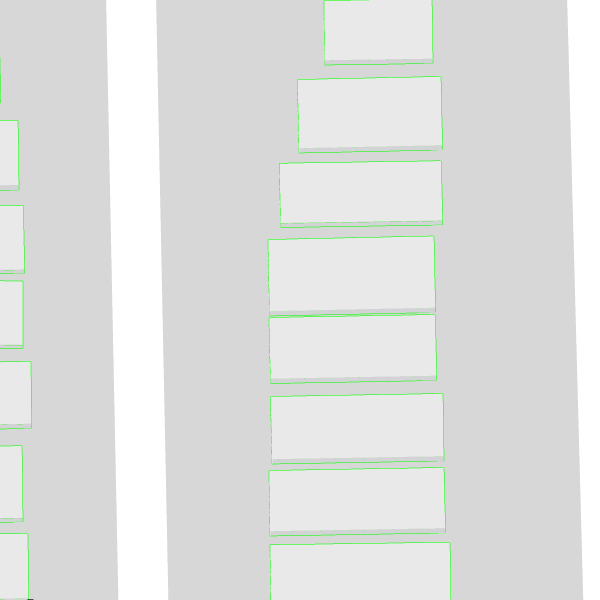
\includegraphics[width=0.328\textwidth]{4-00-1.png}}
	\subbottom[hybrid image\label{fig:eghybrid}]
		{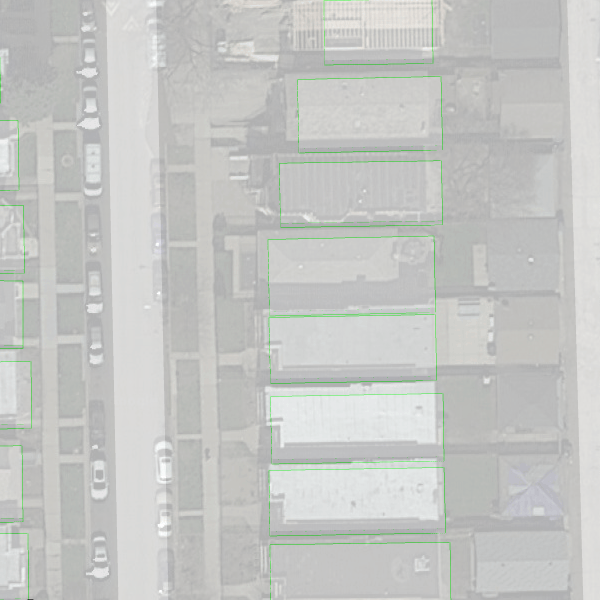
\includegraphics[width=0.328\textwidth]{4-00-2.png}}
    \caption{Example images downloaded through Google Static Maps API. (a) and (b) are obtained directly by the API, with 41.9399708 degrees north latitude, 87.7380649 degrees west longitude of the center (located in Chicago), both width and height 600 pixels, zoom level 20 and scale 1, but different in map types. (c) is obtained by overlaying (a) with (b), with 75\% opacity. It can be clearly seen that the two images cannot match very well.}
	\label{fig:egapimap}
\end{figure}

We would have liked to obtain buildings' coordinates from Google Static Maps API as well, but we find that the API does not provide such information directly. Instead, it gives the styled roadmap images like figure \ref{fig:egroadmap}, where querying coordinates requires further corner detection but the boundaries may be still inaccurate (see figure \ref{fig:eghybrid} for example). Thus, this thesis project, only satellite images from Google Static Maps API are used.

\subsection{OpenStreetMap}\label{apiosm}

OpenStreetMap\footnote{\lstinline{https://www.openstreetmap.org/}} provides an interface that implements a map as a XML format \lstinline{.osm} file. The file contains all the information which can be used to recover the map. When the map's bounding box is given, users can retrieve the latitude and longitude coordinates of the buildings' vertices and roads' central lines within the map. For the usage of OpenStreetMap and the format of the \lstinline{.osm} file, please refer to section \ref{app:apiosm} in appendices.

The coordinates obtained by the API is the original latitude and longitude coordinates of the buildings' vertices, which cannot be directly used for training. We need to convert them to relative pixel coordinates with regards to an given satellite image.

As a matter of fact, every fixed point on the earth can correspond to a unique pixel on the map at a specific zoom level. This projection process can be regarded as a function. Since we have already known the relative pixel coordinates of the image center (half width and half height), the projection for an arbitrary point with given latitude and longitude coordinates can be therefore computed. This process can be described as following equations.
\begin{equation}
	(c_x, c_y) = (\frac{w}{2}, \frac{h}{2}) = f(c_{lon}, c_{lat}, z) + (\Delta_x, \Delta_y),
\end{equation}
\begin{equation}
	(p_x, p_y) = f(p_{lon}, p_{lat}, z) + (\Delta_x, \Delta_y),
\end{equation}
where $f$ is the function that projects latitude and longitude coordinates to global pixel coordinates (see \ref{app:projec} in appendices for more details), $c$ is the image center, $p$ is an arbitrary point, the subscripts $x$, $y$, $lon$, $lat$ mean the relative pixel and longitude and latitude coordinates respectively, $z$ is the zoom level, $\Delta$ is the translation constant from the global to the relative pixel coordinate system. Thus, we have
\begin{equation}
	(p_x, p_y) = f(p_{lon}, p_{lat}, z) - f(c_{lon}, c_{lat}, z) + (\frac{w}{2}, \frac{h}{2}),
\end{equation}
for any arbitrary point $p$.

\subsection{Areas and Buildings}\label{arebui}

As mentioned in section \ref{modmer}, \modelnameshort\ is formed by FPN and PolygonRNN. However, the training phase of these two models requires two different kinds of ground truth dataset.

\paragraph{Areas for FPN}
In subsection \ref{modfpn} we have shown that FPN aims at finding rectangular regions of interests. Thus, training FPN generally requires a relatively large image with several objects in it. When considering our problem, an example of the ground truth can be an area of a city with several bounding boxes. Each box contains a single building, regardless of its tight polygon outline. Figure \ref{fig:egareafpn} gives an example area for training FPN and its visualized ground truth label.

\begin{figure}[!h]
	\centering
	\subbottom[example area\label{fig:egarea}]
		{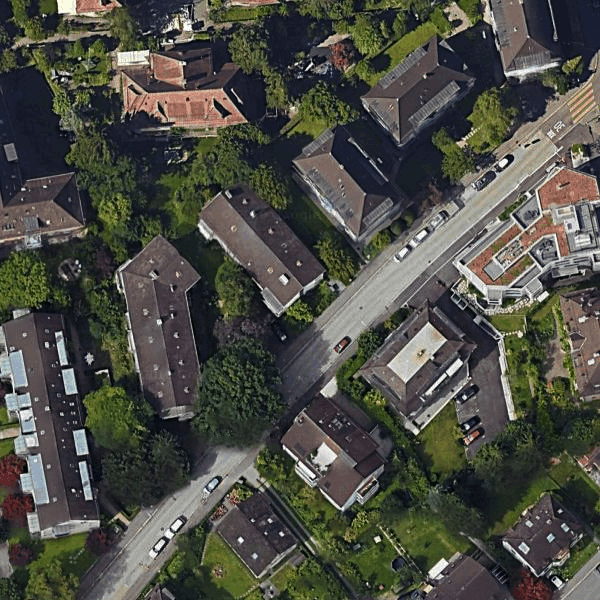
\includegraphics[width=\figfig\textwidth]{4-01-0.png}}
	\subbottom[example area with bounding boxes\label{fig:egareabox}]
		{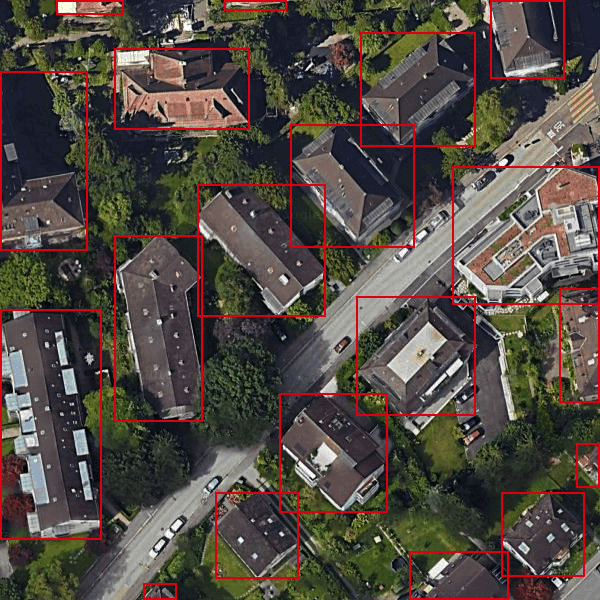
\includegraphics[width=\figfig\textwidth]{4-01-1.png}}
    \caption{An example area in Zurich for training FPN. (a) is the original satellite image obtained by Google Static Maps API. (b) is (a) covered by multiple bounding boxes of buildings, which is visualized based on the ground truth.}
	\label{fig:egareafpn}
\end{figure}

\paragraph{Buildings for PolygonRNN}
In section \ref{modpol} we have mentioned that PolygonRNN can only deal with images with single object, meaning that the bounding box of the object should be first given. Thus, training PolygonRNN generally requires a relatively small image with single object, as well as the information of its polygon outline. When it comes to our problem, an example of the ground truth can be a building with some padding and the pixel coordinates of building's vertices. Figure \ref{fig:egbui} gives example buildings for training PolygonRNN and its visualized ground truth label.

\begin{figure}[!h]
	\centering
	\subbottom[\label{fig:egbui0}]
		{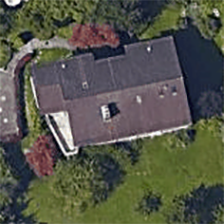
\includegraphics[width=0.243\textwidth]{4-02-0.png}}
	\subbottom[\label{fig:egbui1}]
		{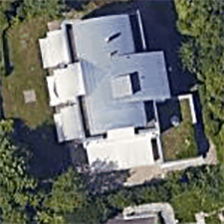
\includegraphics[width=0.243\textwidth]{4-02-1.png}}
	\subbottom[\label{fig:egbui2}]
		{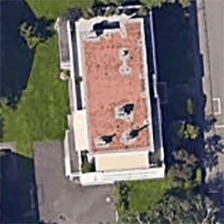
\includegraphics[width=0.243\textwidth]{4-02-2.png}}
	\subbottom[\label{fig:egbui3}]
		{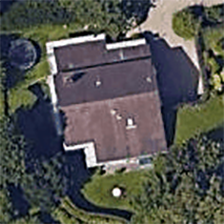
\includegraphics[width=0.243\textwidth]{4-02-3.png}}
	\subbottom[\label{fig:egbui4}]
		{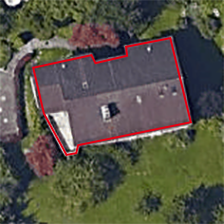
\includegraphics[width=0.243\textwidth]{4-02-4.png}}
	\subbottom[\label{fig:egbui5}]
		{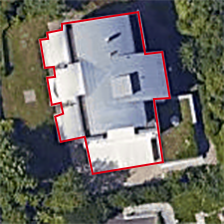
\includegraphics[width=0.243\textwidth]{4-02-5.png}}
	\subbottom[\label{fig:egbui6}]
		{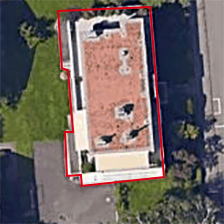
\includegraphics[width=0.243\textwidth]{4-02-6.png}}
	\subbottom[\label{fig:egbui7}]
		{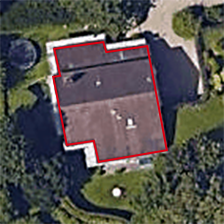
\includegraphics[width=0.243\textwidth]{4-02-7.png}}
    \caption{Example buildings in Zurich for training PolygonRNN. (a)-(d) are the original satellite images obtained by Google Static Maps API. (e)-(g) are (a)-(d) covered by the corresponding polygons' edges, which are visualized based on the ground truth.}
	\label{fig:egbui}
\end{figure}

\subsection{Problems}\label{proble}

Recall that the satellite images and polygons' coordinates are collected from two different sources, the problem of inconsistency may exist. That is to say, the polygon and the actual building we see in the image may not match well in some cases. This inconsistency is mainly reflected in the following aspects.

\begin{figure}[!h]
	\centering
	\subbottom[general shift\label{fig:egshi0}]
		{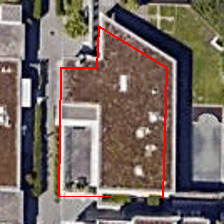
\includegraphics[width=0.243\textwidth]{4-03-0.png}}
	\subbottom[general shift\label{fig:egshi1}]
		{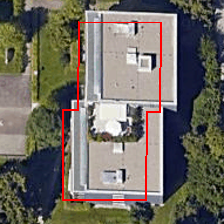
\includegraphics[width=0.243\textwidth]{4-03-1.png}}
	\subbottom[size too small\label{fig:egshi2}]
		{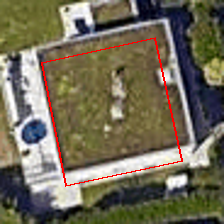
\includegraphics[width=0.243\textwidth]{4-03-2.png}}
	\subbottom[shape too rough\label{fig:egshi3}]
		{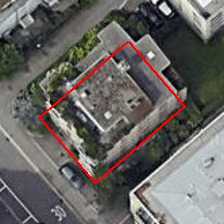
\includegraphics[width=0.243\textwidth]{4-03-3.png}}
	\subbottom[angle issue\label{fig:egshi4}]
		{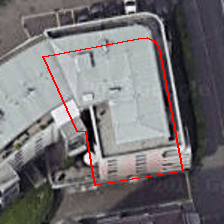
\includegraphics[width=0.243\textwidth]{4-03-4.png}}
	\subbottom[angle issue\label{fig:egshi5}]
		{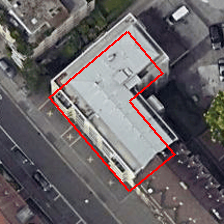
\includegraphics[width=0.243\textwidth]{4-03-5.png}}
	\subbottom[adjacent building\label{fig:egshi6}]
		{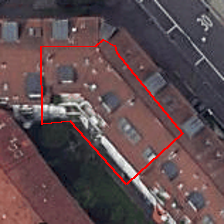
\includegraphics[width=0.243\textwidth]{4-03-6.png}}
	\subbottom[adjacent building\label{fig:egshi7}]
		{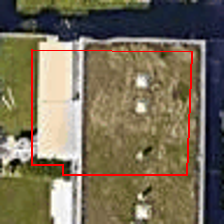
\includegraphics[width=0.243\textwidth]{4-03-7.png}}
    \caption{Problems existed in the ground truth dataset.}
	\label{fig:egshi}
\end{figure}

\paragraph{General Shift}
Figure \ref{fig:egshi0} and \ref{fig:egshi1} give two typical shift examples in the dataset. This shift is generally within the range of 30 pixels, either up and down, or left and right.

\paragraph{Polygon Size and Shape}
Sometimes the polygon size and shape is different from the actual building size as well. This is typically because OpenStreetMap measures the bottom of the building and the aerial image is taken from the top. The roof of the house we see from the top can be different from the floor area. Figure \ref{fig:egshi2} shows a building with a smaller polygon and figure \ref{fig:egshi3} shows a building with a too rough outline.

\paragraph{Angle Issue}
Some tall buildings may suffer from the angle issue. This is because the satellite cannot always be vertically right above the building, so the side of these very high buildings will be photographed. Figure \ref{fig:egshi4} and \ref{fig:egshi5} give two examples.

\paragraph{Adjacent Buildings}
Some adjacent buildings will be very close together, and some even share a common roof. Thus, from the satellite image, it is generally difficult to distinguish the boundaries between them. However, these buildings are separated in the dataset of OpenStreetMap. It means that where there are originally edges between buildings, it looks like there is no edge in the image. This kind of inaccuracy would have  negative effect on the training phase. Figure \ref{fig:egshi6} and \ref{fig:egshi7} give two examples.

\subsection{Adjustments}\label{adjust}
Problems such as too rough polygon shape, angle issue and adjacent buildings are unsolvable unless the data sources can correct themselves. What we can improve is to tackle the general shift and the polygon size problem and make the image-polygon pairs more matching. By observation, we can get to some conclusions for a matching image-polygon pair.

\begin{figure}[!h]
	\centering
	\subbottom[before adjustment\label{fig:egbfradj}]{
		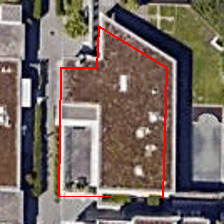
\includegraphics[width=\figfigfigfig\textwidth]{4-04-0.png}
		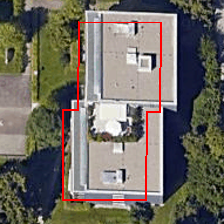
\includegraphics[width=\figfigfigfig\textwidth]{4-04-1.png}
		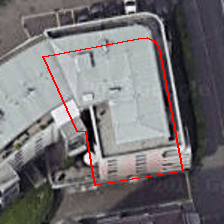
\includegraphics[width=\figfigfigfig\textwidth]{4-04-2.png}
		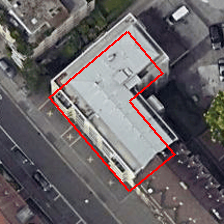
\includegraphics[width=\figfigfigfig\textwidth]{4-04-3.png}
	}
	\subbottom[after adjustment\label{fig:egaftadj}]{
		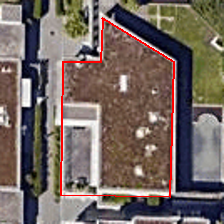
\includegraphics[width=\figfigfigfig\textwidth]{4-04-4.png}
		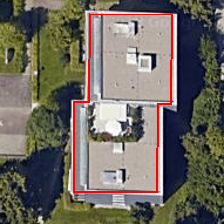
\includegraphics[width=\figfigfigfig\textwidth]{4-04-5.png}
		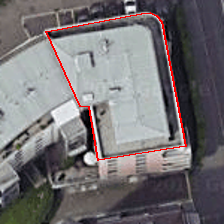
\includegraphics[width=\figfigfigfig\textwidth]{4-04-6.png}
		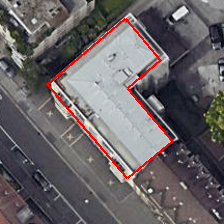
\includegraphics[width=\figfigfigfig\textwidth]{4-04-7.png}
	}
    \caption{Adjustment examples. (a) shows the polygons before adjustment, while (b) shows the polygons after adjustment.}
	\label{fig:egadj}
\end{figure}

\paragraph{Color Variance}
The color variance of image pixels covered by polygon generally reaches the local minimum, because the roof of a building usually has only one color or several similar colors.

\paragraph{Edges}
The polygon edges generally lie within the output of the edge detection (e.g. Sobel, Canny) performed on the image.

\paragraph{Corners}
The polygon vertices can generally match the output of the corner detection (e.g. Harris, SIFT) performed on the image.

Based on these conclusions, we propose a brute force shift adjustment method. Briefly, we resize and translate the initial polygon within a certain range, and traverse all the cases to see where the minimum color variance, maximum edge and corner coverage are reached. This method can address the shift problem to some extent. Figure \ref{fig:egadj} illustrates some examples.

\section{Implementation Details}\label{impdet}

\subsection{Configuration}\label{config}

number of layers
LSTM
polygon anticlockwise

\subsection{Training}

Furthermore, buildings around the edges of areas are typically ignored 

more likely to be incomplete. In this case, the polygon would be clipped by the edges, resulting in new vertices, which can be very hard to compute.
$$(figure placeholder)$$

Although buildings can extract from areas

Therefore, in this project, two different kinds of ground truth dataset are collected separately.
而且独立可以保证训练时的batchsize一致,如果每次训练的Building从area提取,可能会导致每次训练PolygonRNN的batchsize不一致。

\subsection{Prediction}

Beam search

\section{Experiment Results}\label{expres}

Dummy text.

\subsection{Single Building Segmentation}

Dummy text.

\subsection{Buildings Localization}

Dummy text.

\subsection{R-PolygonRNN}

Beam search


\subsubsection{Example Subsubsection}

Dummy text.

\paragraph{Example Paragraph}

Dummy text.

\subparagraph{Example Subparagraph}

Dummy text.

